\begin{figure}[h] 				\subfloat{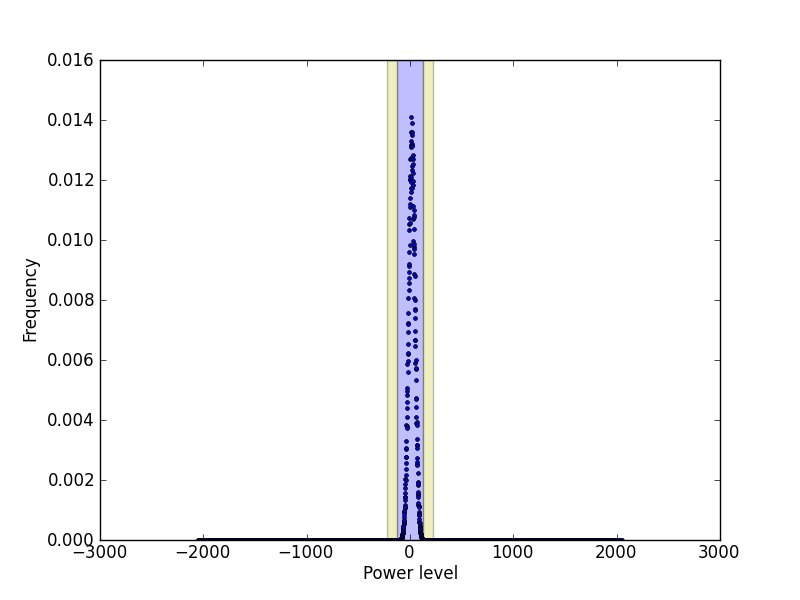
\includegraphics[width=0.5\textwidth]{plots/Stand001Xhist.png}} 				\subfloat{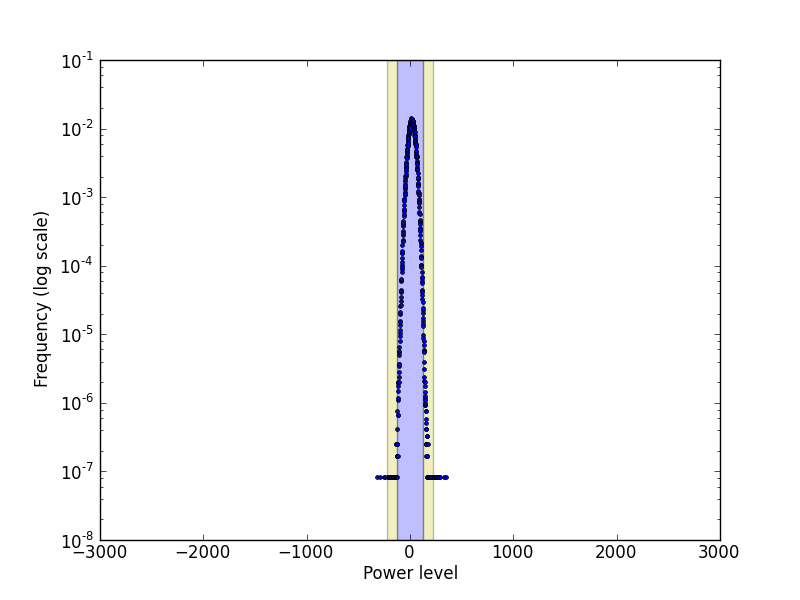
\includegraphics[width=0.5\textwidth]{plots/Stand001Xhist_log.png}} 				\caption{Data from Stand001X. RMS is 34.1188 Samples used : 3792000000. If the RMS is unchanged 99.9896 percent of the samples will lie within [-128,128).  				 With an RMS of 20, 99.9998 percent of the samples will lie within [-128,128).} 				\end{figure} 

\begin{figure}[h] 				\subfloat{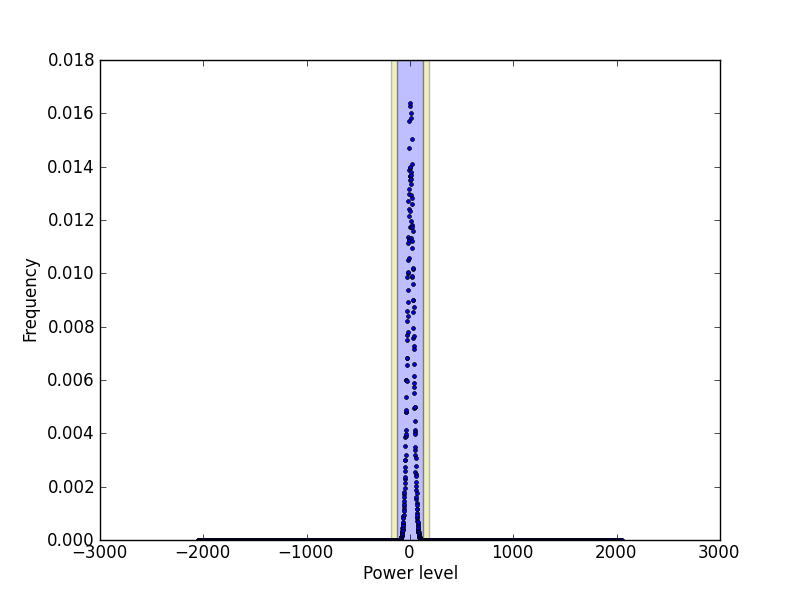
\includegraphics[width=0.5\textwidth]{plots/Stand001Yhist.png}} 				\subfloat{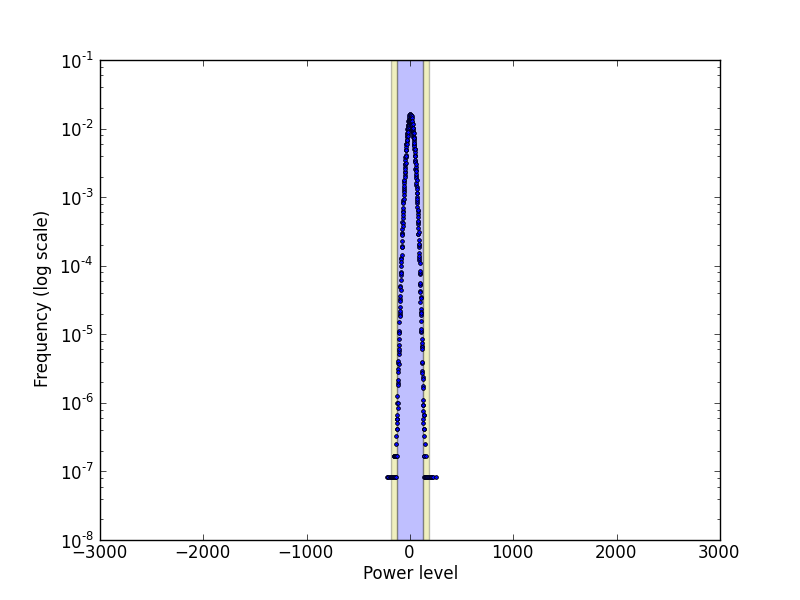
\includegraphics[width=0.5\textwidth]{plots/Stand001Yhist_log.png}} 				\caption{Data from Stand001Y. RMS is 28.5444 Samples used : 3792000000. If the RMS is unchanged 99.9988 percent of the samples will lie within [-128,128).  				 With an RMS of 20, 99.9999 percent of the samples will lie within [-128,128).} 				\end{figure} 

\begin{figure}[h] 				\subfloat{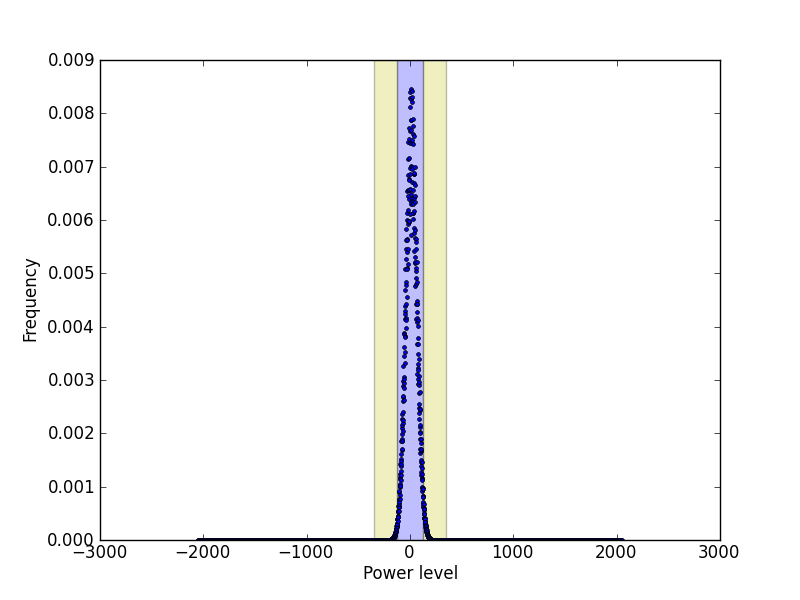
\includegraphics[width=0.5\textwidth]{plots/Stand010Xhist.png}} 				\subfloat{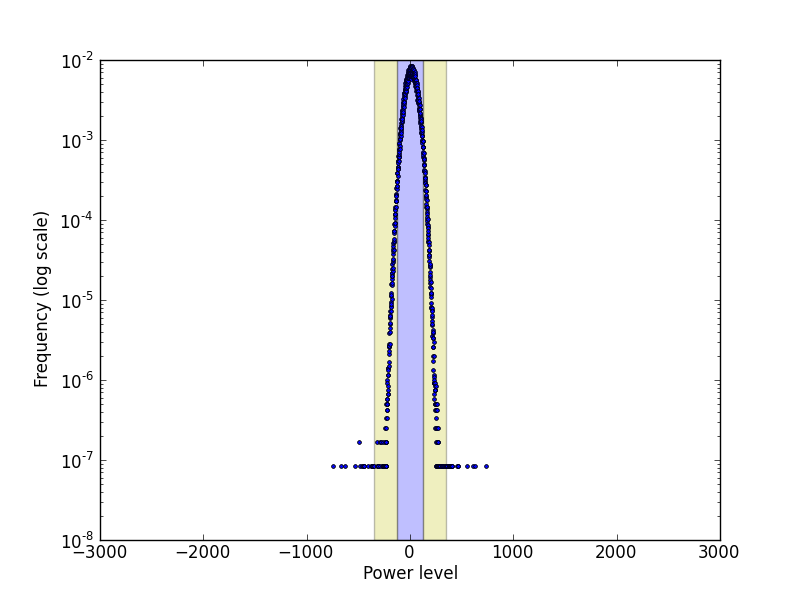
\includegraphics[width=0.5\textwidth]{plots/Stand010Xhist_log.png}} 				\caption{Data from Stand010X. RMS is 55.1743 Samples used : 3792000000. If the RMS is unchanged 98.0064 percent of the samples will lie within [-128,128).  				 With an RMS of 20, 99.9997 percent of the samples will lie within [-128,128).} 				\end{figure} 

\begin{figure}[h] 				\subfloat{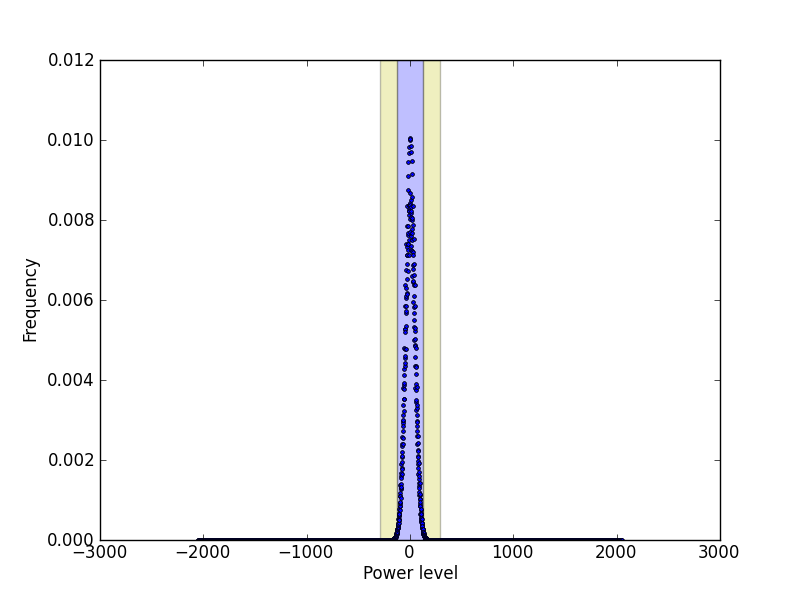
\includegraphics[width=0.5\textwidth]{plots/Stand010Yhist.png}} 				\subfloat{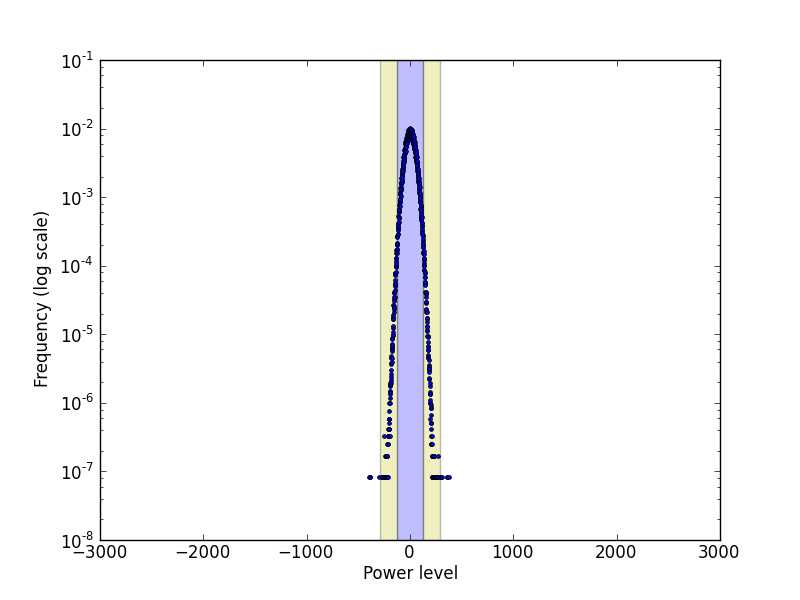
\includegraphics[width=0.5\textwidth]{plots/Stand010Yhist_log.png}} 				\caption{Data from Stand010Y. RMS is 46.1129 Samples used : 3792000000. If the RMS is unchanged 99.4528 percent of the samples will lie within [-128,128).  				 With an RMS of 20, 99.9999 percent of the samples will lie within [-128,128).} 				\end{figure} 

\begin{figure}[h] 				\subfloat{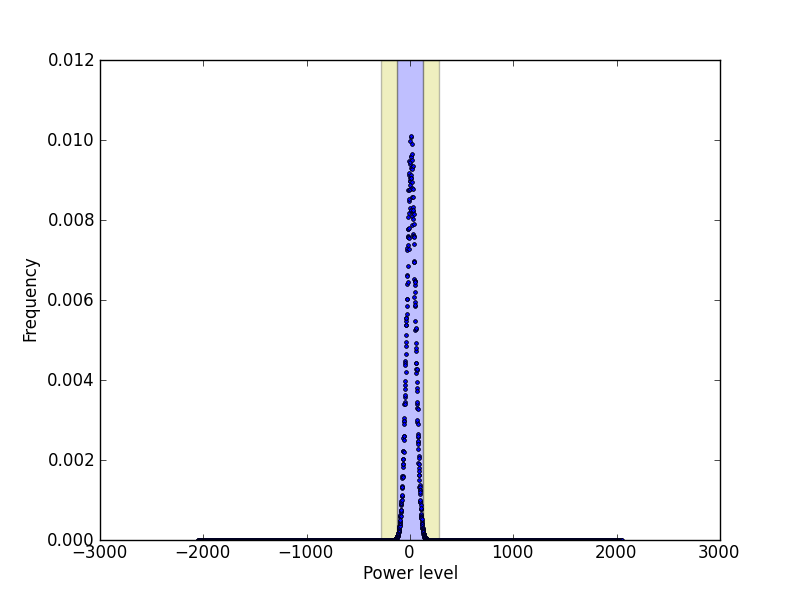
\includegraphics[width=0.5\textwidth]{plots/Stand054Xhist.png}} 				\subfloat{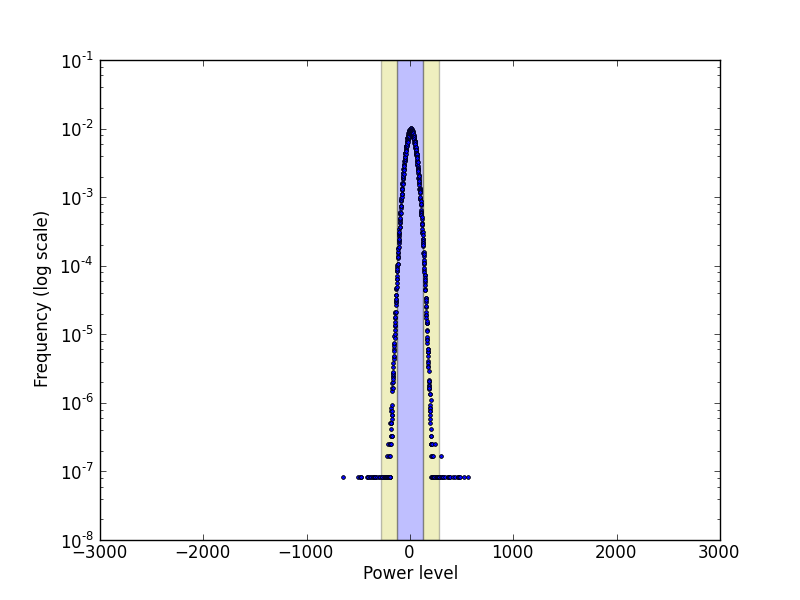
\includegraphics[width=0.5\textwidth]{plots/Stand054Xhist_log.png}} 				\caption{Data from Stand054X. RMS is 43.7177 Samples used : 3792000000. If the RMS is unchanged 99.6627 percent of the samples will lie within [-128,128).  				 With an RMS of 20, 99.9996 percent of the samples will lie within [-128,128).} 				\end{figure} 

\begin{figure}[h] 				\subfloat{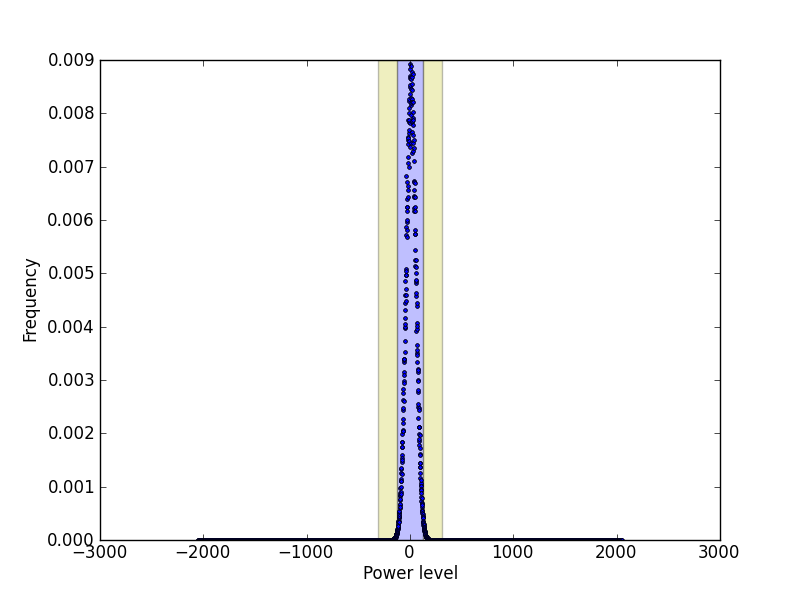
\includegraphics[width=0.5\textwidth]{plots/Stand054Yhist.png}} 				\subfloat{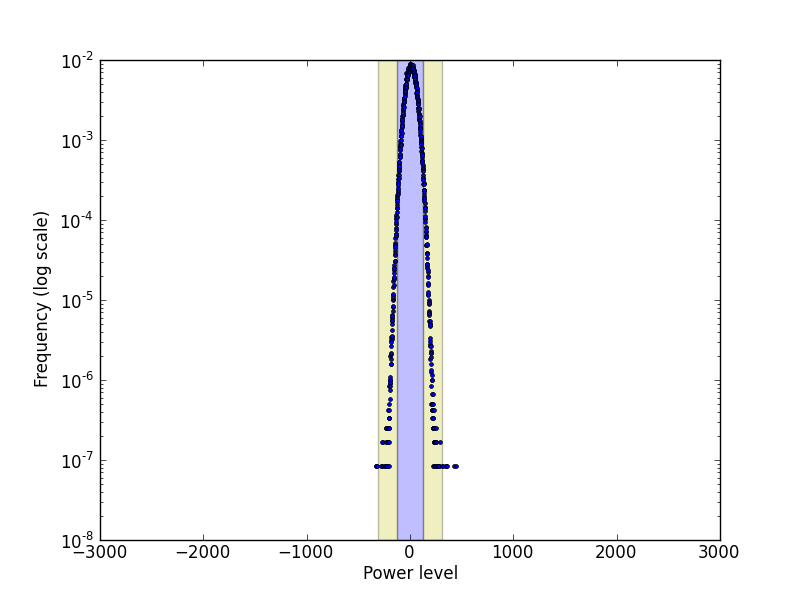
\includegraphics[width=0.5\textwidth]{plots/Stand054Yhist_log.png}} 				\caption{Data from Stand054Y. RMS is 47.8891 Samples used : 3792000000. If the RMS is unchanged 99.2436 percent of the samples will lie within [-128,128).  				 With an RMS of 20, 99.9999 percent of the samples will lie within [-128,128).} 				\end{figure} 

\begin{figure}[h] 				\subfloat{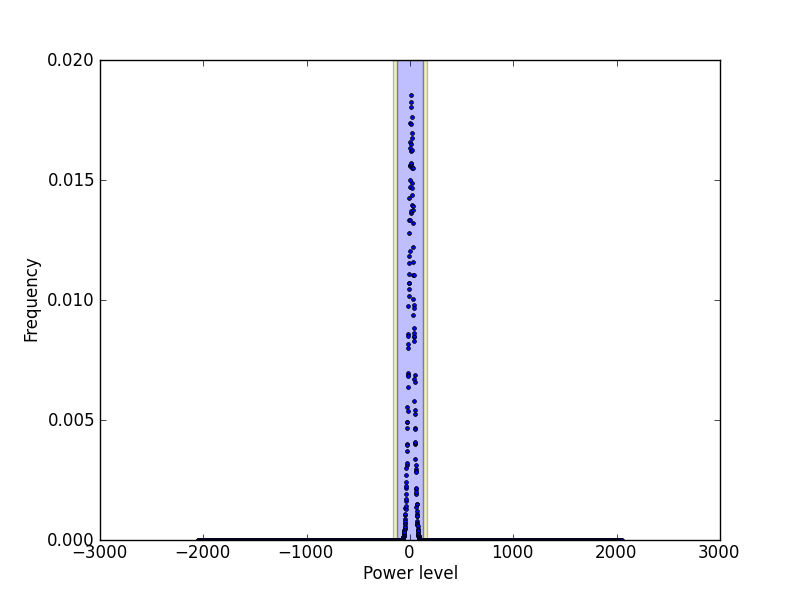
\includegraphics[width=0.5\textwidth]{plots/Stand248Xhist.png}} 				\subfloat{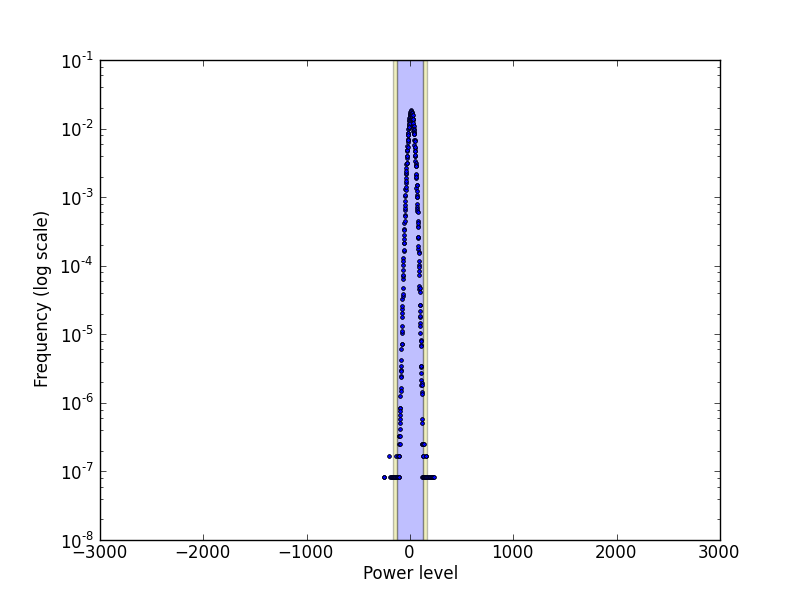
\includegraphics[width=0.5\textwidth]{plots/Stand248Xhist_log.png}} 				\caption{Data from Stand248X. RMS is 26.1238 Samples used : 3792000000. If the RMS is unchanged 99.9996 percent of the samples will lie within [-128,128).  				 With an RMS of 20, 99.9998 percent of the samples will lie within [-128,128).} 				\end{figure} 

\begin{figure}[h] 				\subfloat{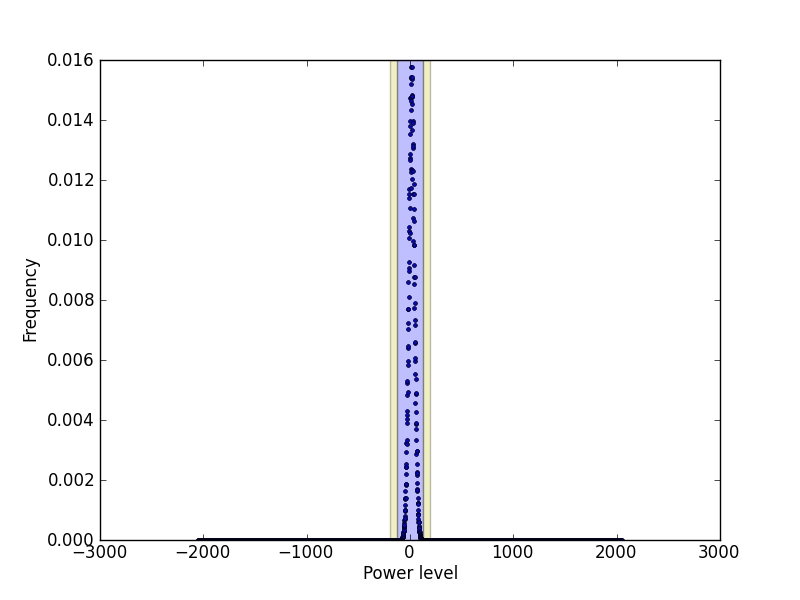
\includegraphics[width=0.5\textwidth]{plots/Stand248Yhist.png}} 				\subfloat{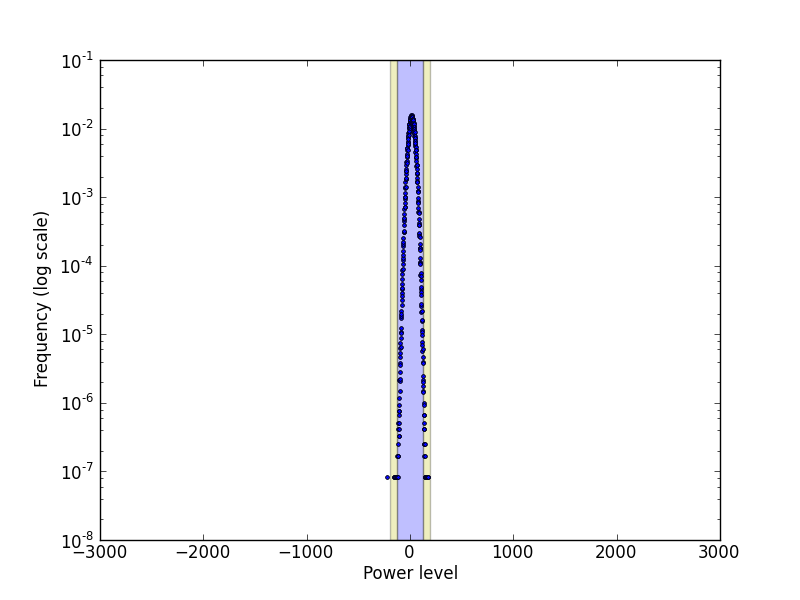
\includegraphics[width=0.5\textwidth]{plots/Stand248Yhist_log.png}} 				\caption{Data from Stand248Y. RMS is 30.7076 Samples used : 3792000000. If the RMS is unchanged 99.9988 percent of the samples will lie within [-128,128).  				 With an RMS of 20, 100.0000 percent of the samples will lie within [-128,128).} 				\end{figure} 

\begin{figure}[h] 				\subfloat{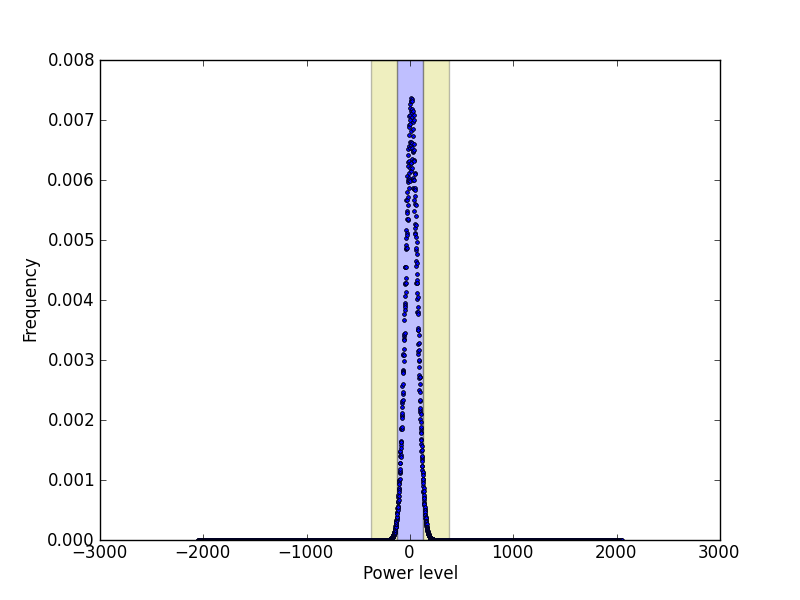
\includegraphics[width=0.5\textwidth]{plots/Stand251Xhist.png}} 				\subfloat{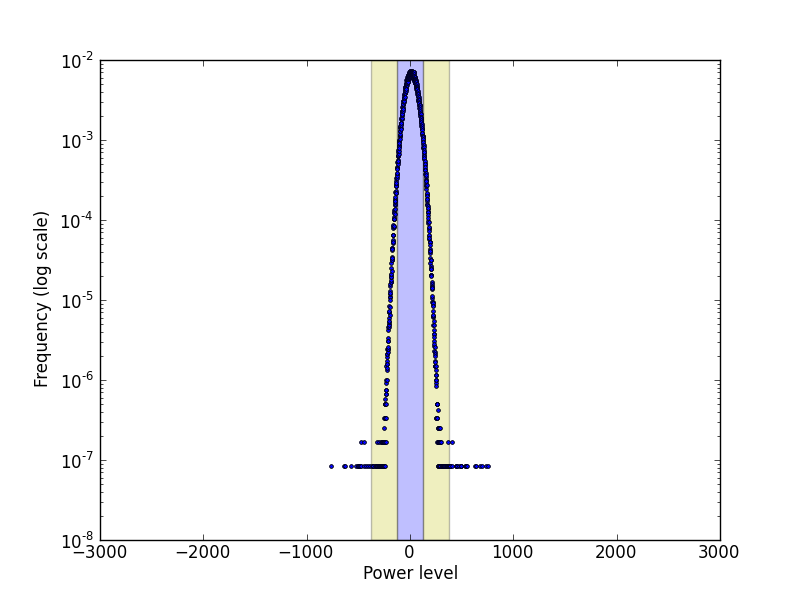
\includegraphics[width=0.5\textwidth]{plots/Stand251Xhist_log.png}} 				\caption{Data from Stand251X. RMS is 58.7564 Samples used : 3792000000. If the RMS is unchanged 97.0939 percent of the samples will lie within [-128,128).  				 With an RMS of 20, 99.9996 percent of the samples will lie within [-128,128).} 				\end{figure} 

\begin{figure}[h] 				\subfloat{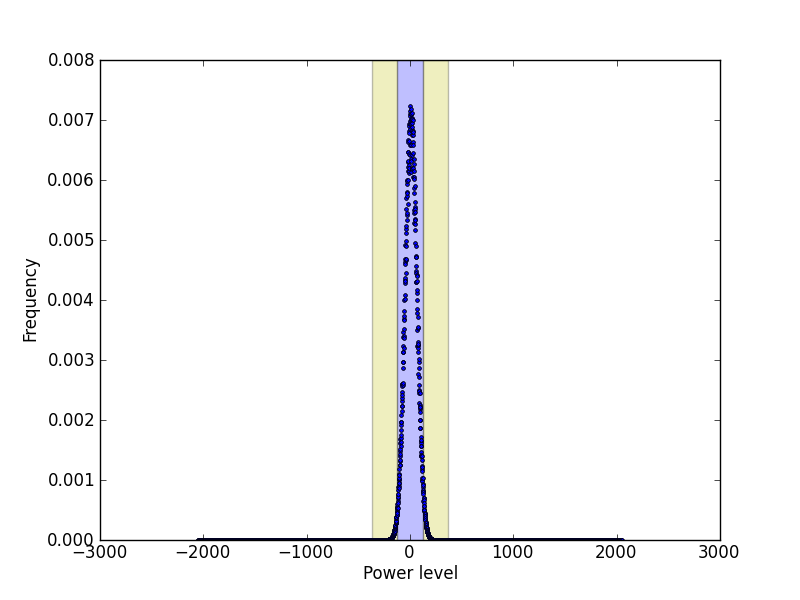
\includegraphics[width=0.5\textwidth]{plots/Stand251Yhist.png}} 				\subfloat{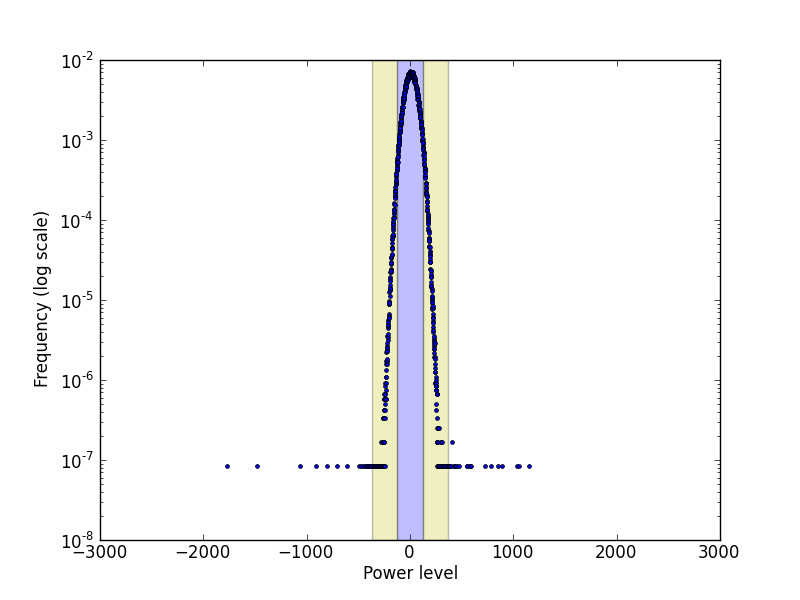
\includegraphics[width=0.5\textwidth]{plots/Stand251Yhist_log.png}} 				\caption{Data from Stand251Y. RMS is 58.0470 Samples used : 3792000000. If the RMS is unchanged 97.2851 percent of the samples will lie within [-128,128).  				 With an RMS of 20, 99.9997 percent of the samples will lie within [-128,128).} 				\end{figure} 

\begin{figure}[h] 				\subfloat{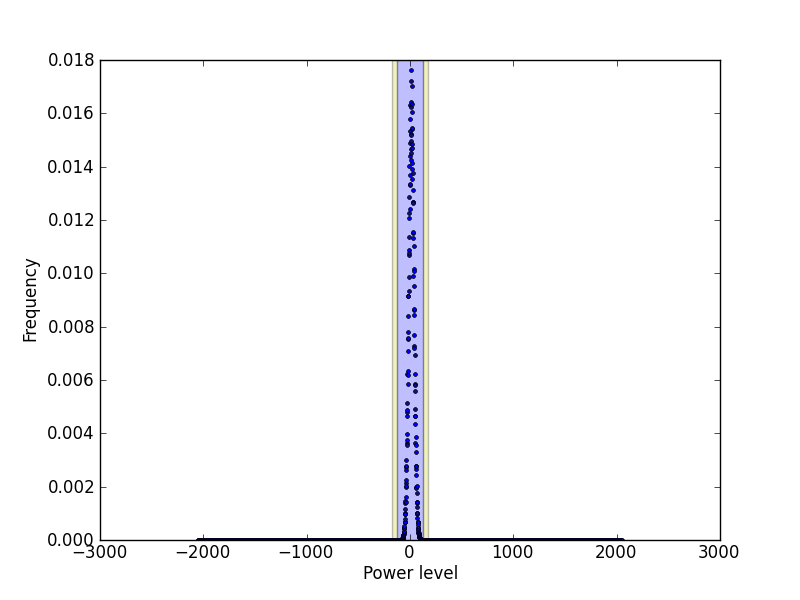
\includegraphics[width=0.5\textwidth]{plots/Stand258Xhist.png}} 				\subfloat{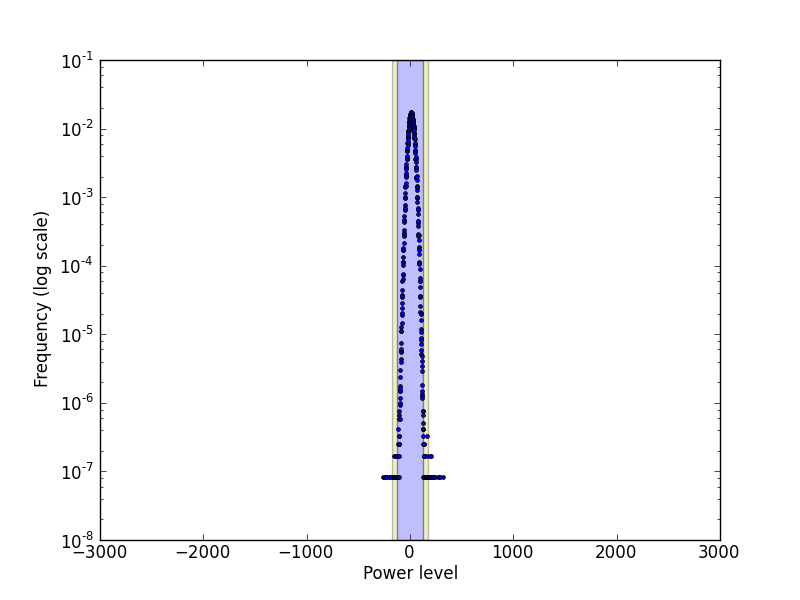
\includegraphics[width=0.5\textwidth]{plots/Stand258Xhist_log.png}} 				\caption{Data from Stand258X. RMS is 27.4041 Samples used : 3792000000. If the RMS is unchanged 99.9993 percent of the samples will lie within [-128,128).  				 With an RMS of 20, 99.9998 percent of the samples will lie within [-128,128).} 				\end{figure} 

\begin{figure}[h] 				\subfloat{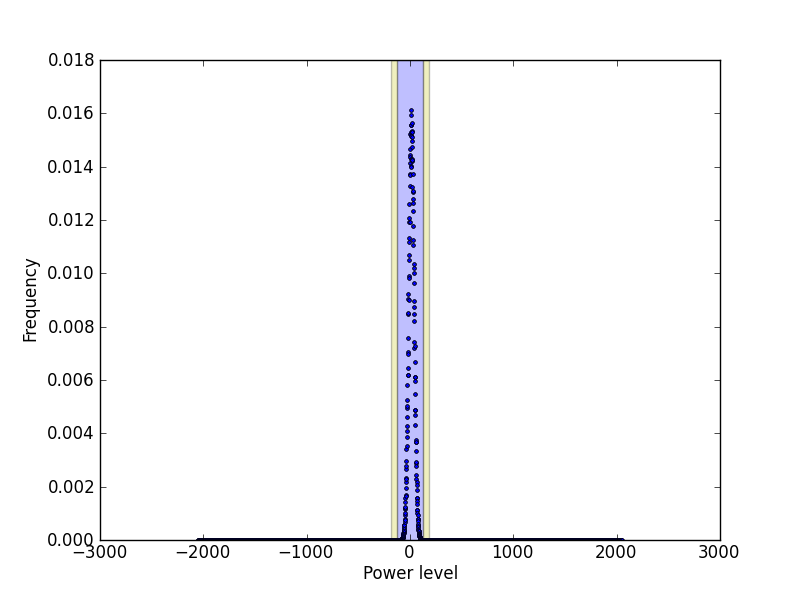
\includegraphics[width=0.5\textwidth]{plots/Stand258Yhist.png}} 				\subfloat{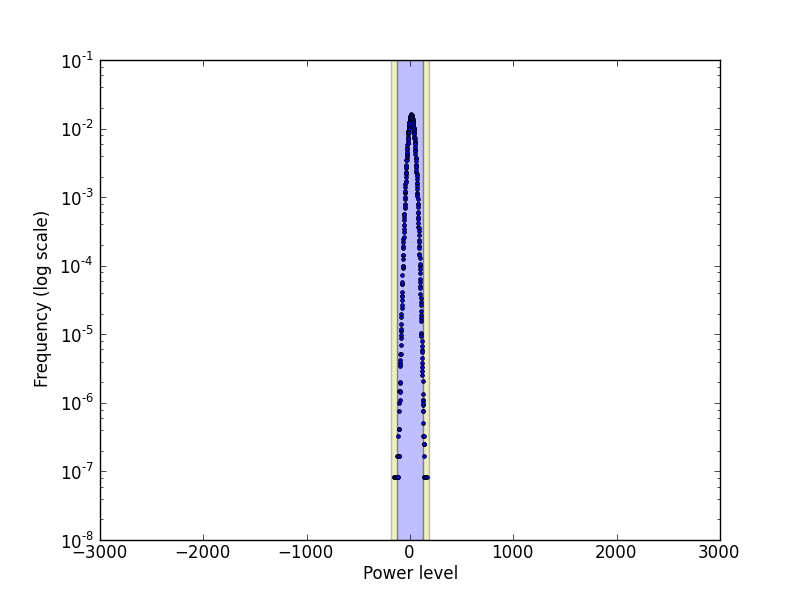
\includegraphics[width=0.5\textwidth]{plots/Stand258Yhist_log.png}} 				\caption{Data from Stand258Y. RMS is 28.3805 Samples used : 3792000000. If the RMS is unchanged 99.9995 percent of the samples will lie within [-128,128).  				 With an RMS of 20, 100.0000 percent of the samples will lie within [-128,128).} 				\end{figure} 

